% !Mode:: "TeX:UTF-8"
\chapter{分支预测解耦前端的设计}

本章首先介绍在高性能处理器设计领域中,前端解耦技术的含义,以及为什么需要对前端解耦,之后详细介绍解耦前端的设计中分支预测相关部分的设计,主要介绍FTQ (Fetch Target Queue) 的功能和设计,FTQ作为连接分支预测部件和取指单元的关键部件,在承担存储取指请求功能的同时也承担了保存分支预测信息和管理后端指令提交信息的功能,通过FTQ能够让以Fetch Block为基本单位的分支预测部件和以单条分支为基本单位的后端流水线进行信息的交互,以实现必要的功能。

\section{香山雁栖湖架构耦合前端简介}

% 还没有介绍BPU的三级覆盖预测和分支历史管理机制
% 还没有介绍IUM
% 也没有讲各个部件SRAM尺寸的改变

在香山雁栖湖架构的设计中,把分支预测和取指单元统称为流水线的前端。相对的以译码为边界,译码和译码之后的流水级统称为后端。在雁栖湖架构的前端设计里,取指单元和分支预测的流水级是耦合的,如图\ref{fig:figure41}所示,这也是以往许多处理器使用的架构,例如BOOM\cite{boom-spec},龙芯\cite{loongson}都是如此。即只有当分支预测和取指单元当前流水级都完成之后,才能够流向下一流水级发送,这会导致分支预测和指令缓存的访问互相阻塞。例如当访问指令缓存发现miss时,即使分支预测已经完成,也仍然需要停下来等待指令缓存从下级缓存中得到回填的数据;同样的当分支预测需要覆盖预测,冲刷流水线时,即使指令缓存已经准备好被访问了,由于流水线被冲刷,暂时没有新的访问请求,也只能够等待分支预测执行。因此在一些公司更高性能的商用处理器,例如Samsung Exynos\cite{samsung-exynos}和IBM z15\cite{ibm-z15}设计中,都会倾向于将这种相互掣肘的耦合关系分开,通过实现解耦前端,可以将大量的前端气泡消除,即将分支预测流水线和取指流水线分离,中间由一个队列连接,这个队列就是FTQ (Fetch Target Queue)。

\begin{figure}[htb]
	\centering
	\setlength\tabcolsep{3pt}  % 同一行中的图片间隔
	\vspace{5pt} % 图片上部的空白,如果太小的话,图片顶部会与正文内容十分接近
	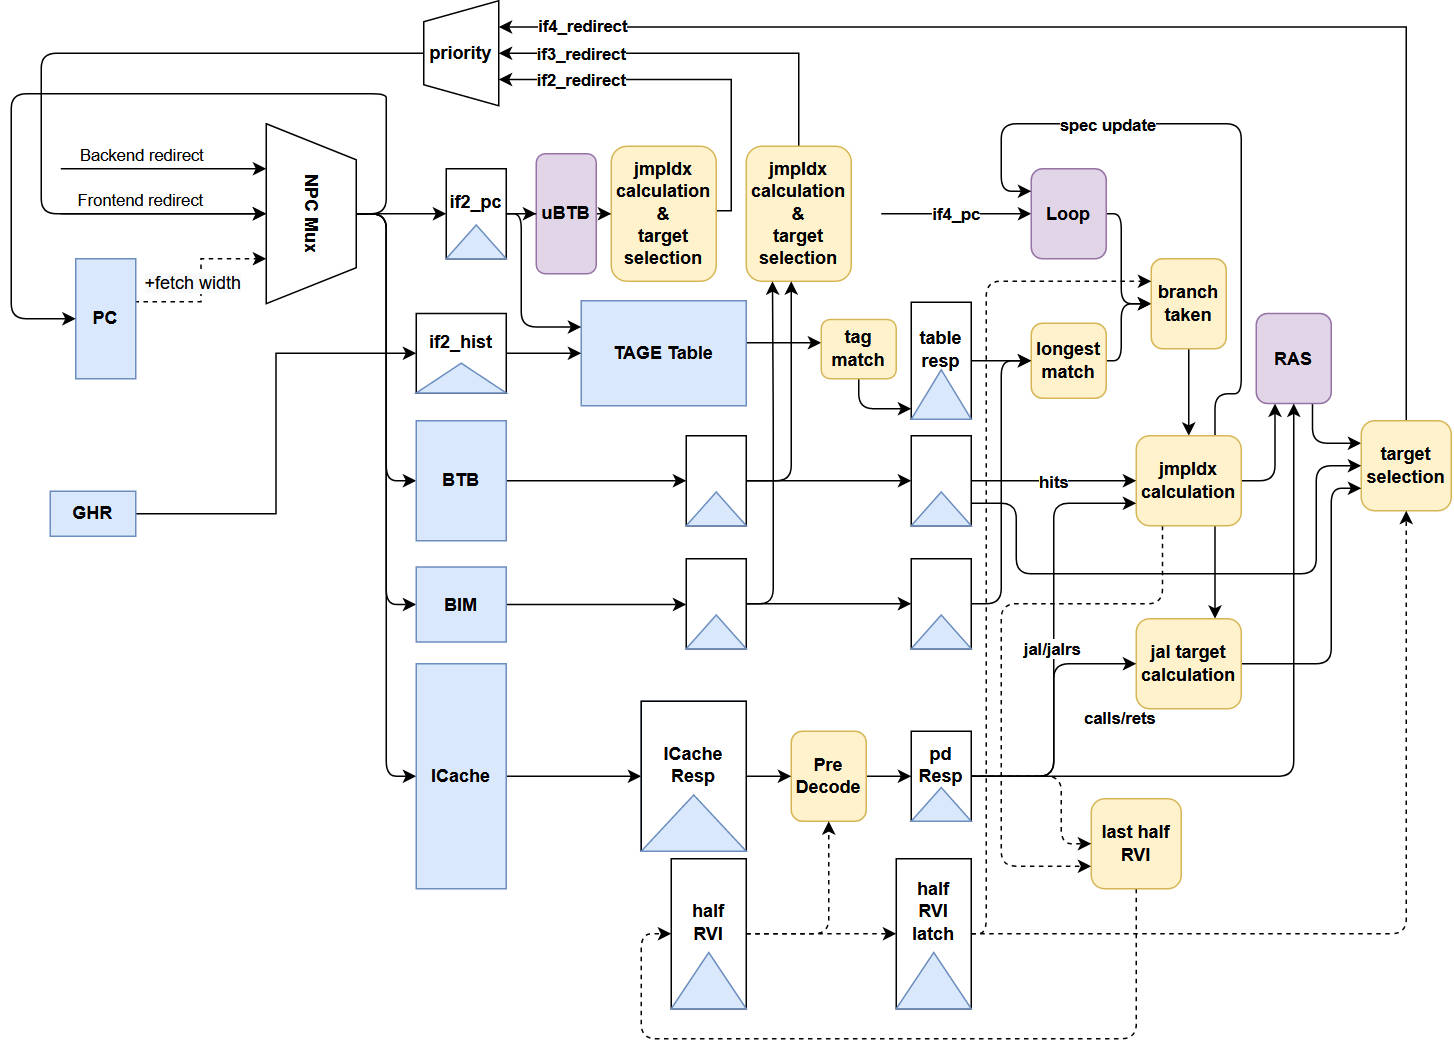
\includegraphics[width=1\textwidth]{yqh-IFU-BPU.jpg}
	\caption{香山处理器雁栖湖架构分支预测与取指架构图}
    \label{fig:figure41}
\end{figure}

\section{通过FTQ实现前端解耦}

通过将分支预测流水线和取指流水线解耦开,通过FTQ连接,如图\ref{fig:figure21}所示,就能够将分支预测和取指单元变成类似于生产者和消费者的关系:分支预测作为生产者,负责不断地预测当前PC下一拍的取指PC,而无需关心指令缓存是否miss,只需要将相关的取指请求放入FTQ之中。而取指单元作为消费者,负责不断地从FTQ中顺序取出取指的请求,访问指令缓存得到指令码,将它传给后端。由于在指令缓存miss时,分支预测仍旧会不断地往FTQ中送入取指请求,因此当分支预测冲刷流水线时,取指单元也不用等待,可以继续取出FTQ中之前存储的取指请求,继续访问指令缓存。如此便能减少前端大量不必要的气泡,提高前端的供指效率,也会对整体架构的性能有一定的正面影响。

FTQ并不是一个简单的队列,除了储存分支预测部件预测需要取指的Fetch Block外,在取指单元需要取指时给出合适的取指地址,但此时对应的被取指的block并不会直接出队,假设将取指地址发送给取指单元后立即将对应的block出队,则当有分支指令误预测发生时,无法恢复到正确的指令执行路径上,因为仅通过分支误预测的指令地址无法判断它属于哪一个Fetch Block中,无法对分支预测部件进行恢复,同样的,在有指令提交时,也无法判断被提交的指令属于哪个Fetch Block,则无法对分支预测部件进行更新。因此FTQ在将取指地址发送给取指单元后,仍要暂时保存这些Fetch Block,以及用于分支预测恢复和更新的相关数据,以保证分支预测的正常运作。

也正因此,FTQ同时连接着分支预测、取指单元和后端执行单元,除了用于将分支预测和取指单元解耦,还负责记录所有在流水线中执行指令的状态,保存分支预测信息和指令预译码信息。以及负责接收从后端和取指单元传来的redirect信息,包含分支误预测和指令replay请求,并给分支预测和取指单元发送恢复信号和必要信息。FTQ的每个项代表了一个Fetch Block,当FTQ中的一个block里所有的有效指令都被提交后,FTQ会给分支预测发送commit信息,用于训练分支预测器。

\subsection{FTQ中的存储结构}

由于FTQ不止要向取指单元提供取指地址,还要管理分支预测部件的恢复和更新,以及所有指令在流水线中的执行状态,因此相比于普通的只有头尾指针的队列,在FTQ中有4个指针,分别代表所有指令在流水线中的不同进度,用于控制分支预测部件的更新和误预测时整个前端流水线的恢复。

\begin{enumerate}
	\item bpuPtr:类似队尾指针,当分支预测产生新的取指请求时从这个指针指向的位置入队
	\item ifuPtr:指向最近一次发送给取指单元的block
	\item ifuwbPtr:指向最近一次从取指单元写回预译码信息的block
	\item commPtr:类似队头指针,指向最近一次被提交的block
\end{enumerate}

FTQ是一个循环队列,其中使用的指针都是FtqPtr类的实例,设计参考了《超标量处理器》中的设计\cite{superscala}。每个指针有flag和value 2个值,其中value代表这个指针指向队列中第几个元素,而flag代表的是这个指针在哪一次遍历,如图\ref{fig:figure42}所示,图\ref{fig:figure42}(a)中tail指向第4个元素,head指向第2个元素,tail和head都在同一次遍历中,flag都为0,灰色代表了队列中有效的项。而图\ref{fig:figure42}(b)中继续入队出队后,head指向了3,而tail已经完成了一次遍历,再次从0开始向后遍历到了1,此时head和tail不在同一次遍历中,head的flag为0,而tail的flag为1,此时队列中的有效项不在head和tail之间,而是相反的。图\ref{fig:figure42}(c)中当head也完成了一次遍历,回到0时,此时head和tail的flag再次变为相同,都为1,有效项也变回了head和tail之间的项。使用这种方法,就可以很好的解决循环队列中不知道head和tail在哪一轮遍历中的问题。除了FTQ以外,这种数据结构在香山的其他部件中也有广泛的应用。

\begin{figure}[htb]
	\centering
	\setlength\tabcolsep{3pt}  % 同一行中的图片间隔
	\vspace{5pt} % 图片上部的空白,如果太小的话,图片顶部会与正文内容十分接近
	\begin{tabular}{ccc}
		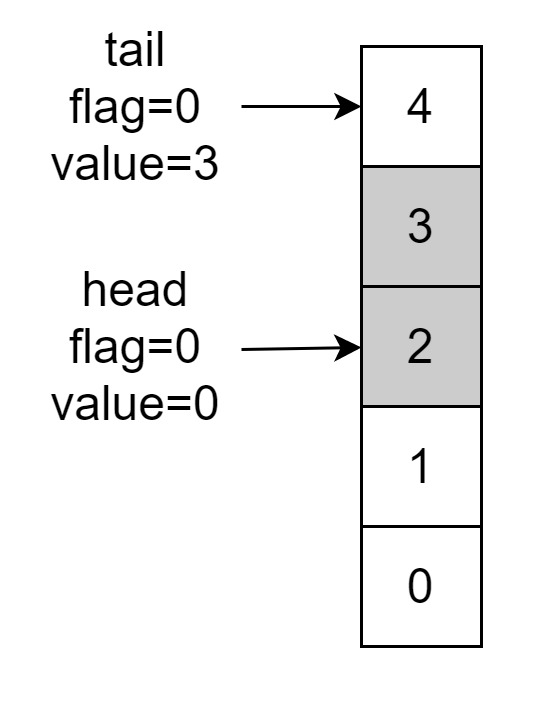
\includegraphics[width=0.23\textwidth]{queue_ptr_a.jpg} &
		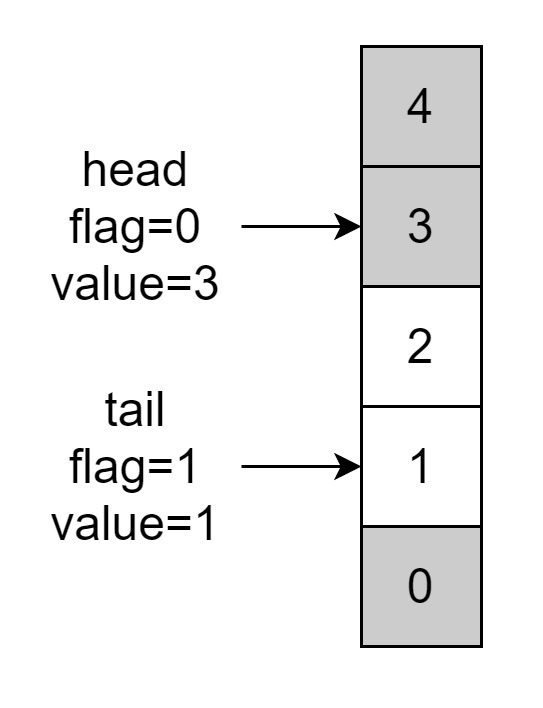
\includegraphics[width=0.23\textwidth]{queue_ptr_b.jpg} &
		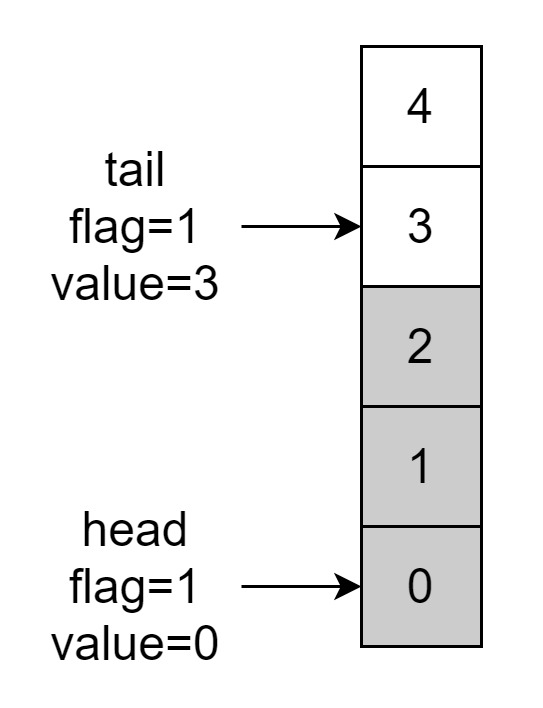
\includegraphics[width=0.23\textwidth]{queue_ptr_c.jpg} \\
		(a) & (b) & (c) \\[1ex]
	\end{tabular}
	\caption{通过flag表示head和tail指针是否在同一轮遍历中,其中图(a)和图(c)在同一轮遍历中,图(b)不在同一次遍历中}
	\label{fig:figure42}
\end{figure}

由于FTQ需要负责分支预测的恢复和更新,因此除了需要存储基本的Fetch Block以外,还需要存储一些必要的信息,用于维护和管理分支预测和取指单元。主要是在对分支预测时产生的预测信息,以及取指单元在取完指令进行预译码之后的信息,用于在更新和误预测恢复时指导FTQ给出正确的Fetch Block用于分支预测部件。在FTQ中的表项需要存储的信息分为几类,分别存在不同的寄存器堆中,大致分为以下几类:

\begin{itemize}
	\item PC相关信息。主要存储block的起始地址,以及一些其他的信号位。在分支预测有新的取指请求,以及分支预测redirect时写入。
	\item redirect分支预测重定向相关信息。分支预测在redirect恢复时需要的一些信息,例如RAS栈顶元素和栈顶指针,全局历史指针等。在分支预测最后一个流水级发送时写入
	\item 分支预测meta信息。用于保存所有预测器在预测时产生的meta信息,是一个很长的Unsigned Int,将所有的meta信息都转成Unsigned Int拼接起来,拼接和拆分由Composer组件负责。在分支预测最后一个流水级fire时写入
	\item FTB表项。存放从分支预测传来的FTB表项。在分支预测最后一个流水级发送时写入,用于判断是否出现false\_hit,以及在指令提交时判断表项有无改变,产生新的表项。
	\item 预译码信息。用来存储取指单元写回的预译码信息,用于在指令提交时生成新的FTB表项。
\end{itemize}

取指单元在取指时是按照Fetch Block来取指的,但在指令执行完毕提交时,并非严格按照Fetch Block提交,但只有当一个Fetch Block中所有的指令都提交后,这个block才能够提交给分支预测更新,否则其中的指令信息可能会不完全或者错误,这就需要一个管理FTQ中所有block中指令状态的队列,即commitStateQueue,commitStateQueue队列长度与FTQ存储Fetch Block的队列长度相同,用于表示每个表项代表的Fetch Block中所有指令的状态,有invalid,valid,commited三个状态。当某个block中只有invalid和commited时,代表这个block中所有的有效指令都已提交,这时就可以以整个block为单位,给分支预测发送更新信号。当有redirect信号时,这个队列也要进行恢复。

此外还有一个表示FTB hit状态的队列entry\_hit\_status,用来表示Fetch Block在FTB中的hit状态,有not\_hit,hit和false\_hit三个状态。其中false\_hit状态表示的是在查找FTB时hit了,但是Fetch Block中有分支指令的信息与预译码不符,例如在block中的offset不同,分支指令的类型错误等情况。出现这种情况原因是因为在FTB中存储的tag不是完整的tag,当程序达到了一定的大小,便有可能出现别名的情况,即两个不同的Fetch Block的tag相同,但是其中的分支信息完全不同。但是这种情况比较少出现,对性能影响有限,而不使用完整的tag可以一定程度上减少SRAM的大小。

在FTQ入队时每个表项都只会是hit或者not\_hit的状态,但是在取指单元写回预译码信息后,FTQ会根据预译码信息将部分hit信号修改为false\_hit。

保存FTB hit的状态可以用于分支历史的更新,以及控制FTQ发送更新信息给FTB的时机。由于在第三章中提到,FTB在预测时没有hit,那么更新前就要先查找一遍FTB后再写入,需要2个周期,但是存在连续几个周期都有block被提交的情况,因此FTQ要根据FTB是否hit,来决定什么时候给FTB发送更新请求。

\subsection{FTQ的行为逻辑}

本小节详细介绍在南湖架构中的FTQ的相关行为逻辑,以及与其他部件是如何交互的。

首先当分支预测S1完成后得到一个初步的预测结果,会将刚才预测的PC传给FTQ,如果FTQ未满,则会将其入队,同时bpuPtr递增。如果队满了则会阻塞分支预测的流水线,而由于FTQ满意味着前端供指充足,因此这种阻塞不会影响处理器的整体性能。FTQ中有bypass逻辑,如果取指单元已经准备好访问指令缓存,那么下一周期就可以将这个取指请求送往取指单元访问指令缓存。否则则储存在FTQ中。

由于在S1预测时还没有得到FTB等其他预测器的返回结果,因此S1时入队的FTQ项中有效的只有PC相关的信息。S1入队后FTQ会返回指向新入队表项的指针,在分支预测全部结束之后,会将剩余的信息补充到对应的表项中。之所以在S1预测结束后就要急于将取指请求发往FTQ,是由于如果等到S3所有的分支预测结束后再发往FTQ,则会增加整个前端流水线的深度,导致分支误预测的惩罚周期变长。

由于分支预测采用的是覆盖预测机制,即当后面的流水级中更准确的预测器预测结果与前面的流水级不同时,以后面的流水级为准,并且冲刷流水线,恢复之前错误的取指请求。因此FTQ在分支预测冲刷流水线时,相应的要将bpuPtr,ifuPtr和ifuwbPtr都恢复到正确的位置。同时由于这时候可能已经有错误的请求发往取指单元了,因此也要给取指单元发相应的恢复请求。

在取指请求发送给取指单元,取指单元取回指令完成预译码后,要将预译码的信息传回给FTQ储存起来,同时要判断一些简单的误预测,例如jump指令被预测为不跳转等情况。同时还会修改commitStateQueue的状态,将对应的项改为valid,代表指令已经送去后端流水线执行,但是还没有提交。

FTQ也要将分支预测的结果传给后端执行单元,在分支指令执行后要再次和预测结果比较,最终确定分支指令有没有误预测。

取指单元和后端执行单元都有可能发现分支误预测,误预测时需要给FTQ发送redirect分支预测重定向信号,假如两者同时发现误预测,由于正在执行单元的分支指令指令序比在取指单元的分支指令早,因此以后端的redirect信号为优先。

FTQ收到redirect信号之后,会拿到取指单元或后端发回的出现了误预测指令的FTQ表项的指针,根据这个指针将相关的数据从FTQ中取出,进行处理后向分支预测发送redirect信号,恢复分支预测器以及分支历史。如果redirect来自后端,那么也要给取指单元发redirect信号,因为取指单元也需要恢复错误的取指。同时需要恢复bpuPtr,ifuPtr和ifuwbPtr到redirect发回的指针加1的位置,因为这条误预测的指令以及之前的指令仍然是要提交的。同时需要将误预测指令所在的Fetch Block中所有在这条指令之后的指令状态都置为invalid。

当有指令提交时,FTQ需要将对应的指令的状态改为commited,当一个block中的所有指令状态是invalid或commited,并且其中有跳转的指令,或者曾在FTB中命中,那么block就可以向分支预测提交。提交时会从FTQ中取出对应的预译码信息,meta信息等,送往分支预测用于更新预测器的训练数据。

% FTQ会接收BPU s2和s3的信号,当分支预测部分有redirect时,FTQ中也要将指针恢复到正确的位置

% 每次有取指请求入队时,FTQ需要给分支预测返回新入队的项的bpuPtr,在分支预测redirect时需要用这个指针进行恢复。

% 取指请求在分支预测S1 fire和S2,S3 redirect的时候发送给FTQ

% FTQ中的存储结构(或者说FTQ表项中的组成部分)主要有:

% update\_target
% cfiIndex\_vec
% mispredict\_vec
% pred\_stage

% entry\_fetch\_status。用来表示FTQ项对应的取指状态

% entry\_hit\_status。用来表示FTQ项在FTB的hit状态,有not\_hit,hit和false\_hit。

% 当分支预测s2和s3需要redirect时,FTQ要负责把bpuPtr和ifuPtr都移动到正确的位置。同时把redirect信号发给IFU,IFU对之前的错误的取指进行恢复

% FTQ有bypass操作,如果上一拍BPUfire,且ifuPtr等于当前的bpuPtr,就直接将最新的取指请求发给IFU

% FTQ还要接收从IFU写回的信息,在取指请求发给IFU,IFU取回指令码,并预译码之后,会将预译码信息传回FTQ保存起来,同时IFU还会检测是否有明显的误预测,如果有也会发给FTQ,由FTQ给分支预测发送误预测恢复信号。并将commitStateQueue有效的指令状态修改为valid

% 写回后还会和之前保存的FTB entry进行判断,有没有false\_hit,当FTB hit,但是预译码结果和FTB entry中的结果不一致时,则认为是出现了false\_hit的情况,具体可能有是分支不是分支,是跳转不是跳转,以及跳转目标地址的offset不同

% FTQ还要将指令信息传给后端,由后端执行时再做一次判断,决定是否误预测

% 当后端发现误预测指令时,后端回发回误预测信号和误预测指令所在block的FtqPtr,FTQ根据这个指针去读取ftq\_redirect\_sram和ftb\_entry\_mem中的数据,将这些数据进行处理后发送回分支预测,并更新分支历史

% IFU发的redirect也和后端的处理方式类似

% RedirectGen。接收后端发来的信息,生成redirect信号

% 恢复指针和state queue。在有误预测时,需要恢复FTQ的指针和状态队列,redirect的来源有后端和IFU,同时发redirect时以后端的优先,在redirect发生时,无论是后端还是IFU,都会发回发生redirect的block在FTQ中对应的指针,需要将bpuPtr,ifuPtr,ifuwbPtr都恢复到redirect 指针加1的位置,因为误预测的指令所在的block也是需要提交的。同时需要将block中误预测指令之后的所有指令的状态都置为invalid。

% 后端发redirect时,FTQ不光要给分支预测发redirect,也要给IFU发

% 每当有指令提交时,FTQ需要将对应指令的状态修改为commited

% 当一个block中的所有指令状态是invalid或commited,并且其中有跳转的指令,或者曾在FTB中命中,那么block就可以向分支预测提交了。提交时会把ftq\_pc\_mem,ftq\_pd\_mem,ftq\_redirect\_sram,ftq\_meta\_1r\_sram,ftb\_entry\_mem中commPtr中对应的数据都取出来,用于生成传给分支预测的分支预测训练数据。

% FTQ会控制发送commit的频率,如果某次更新FTB需要先查找FTB再写入,那么FTQ就会将之后的commit请求延后,等到FTB准备好下一次更新时再发送。

% FTB中表项的更新逻辑由FtbEntryGen中实现

% FTQ还有一些支持指令预取的逻辑




% 雁栖湖架构的分支历史是按照一个packet 1 bit的,南湖架构是每条分支1 bit

\section{本章小结}

本章首先介绍了雁栖湖架构的前端流水线设计,之后介绍在高性能处理器设计中,分支预测与取指单元耦合带来的影响,为什么在南湖架构中决定使用解耦前端的设计,以此引出解耦前端的设计思路,以及FTQ这个模块的意义。之后介绍了FTQ是如何实现前端解耦的,以及其基本的功能。再进一步介绍FTQ中存储的分支预测信息和指令信息的组织结构,以及为什么要这样设计。最后再详细介绍了FTQ和分支预测、取指单元、后端执行单元的交互逻辑。除香山处理器外,其他类似架构的处理器在实现时也可以参考这种设计思路。
